\documentclass[aspectratio=169,10pt]{beamer}

% Theme & Colors
\usetheme{Madrid}
\usecolortheme{whale}
\setbeamertemplate{navigation symbols}{}
\setbeamertemplate{footline}[frame number]
\setbeamerfont{frametitle}{size=\large,series=\bfseries}

% Packages
\usepackage[utf8]{inputenc}
\usepackage[T1]{fontenc}
\usepackage{graphicx}
\usepackage{amsmath,amssymb}
\usepackage{booktabs}
\usepackage{tikz}
\usetikzlibrary{arrows.meta,positioning,shapes.geometric,calc}
\usepackage{xcolor}
\usepackage{multicol}

% Custom colors
\definecolor{probpose}{RGB}{41,128,185}
\definecolor{accent}{RGB}{231,76,60}
\definecolor{success}{RGB}{39,174,96}
\definecolor{warning}{RGB}{243,156,18}

% Title info
\title[ProbPose]{\textbf{ProbPose: A Probabilistic Approach\\to 2D Human Pose Estimation}}
\subtitle{Paper Review --- CVPR 2025\\{\small Miroslav Purkrabek \& Jiri Matas}}
\author{Ardityo Cahyo \and Salman Rachmadi \and Ahmad Taufiq}
\institute{Paper Review: Purkrabek \& Matas (CVPR 2025)}
\date{}

\begin{document}

% ============================================================
% TITLE
% ============================================================
\begin{frame}
\titlepage
\end{frame}

% ============================================================
% OUTLINE
% ============================================================
\begin{frame}{Outline}
\begin{enumerate}
    \item Apa itu Human Pose Estimation?
    \item Bagaimana cara kerjanya? (Top-Down + Heatmap)
    \item Masalah yang belum terselesaikan
    \item ProbPose: Solusi probabilistik
    \item Evaluasi baru: CropCOCO \& Ex-OKS
    \item Hasil eksperimen
    \item Demo
\end{enumerate}
\end{frame}

% ============================================================
% PART 1: WHAT IS POSE ESTIMATION
% ============================================================
\section{Human Pose Estimation}

\begin{frame}{Apa itu Human Pose Estimation?}
\begin{columns}
\begin{column}{0.5\textwidth}
\textbf{Tujuan:} Menemukan lokasi sendi-sendi tubuh manusia dalam gambar.

\vspace{1em}
\textbf{Output:} 17 titik koordinat $(x, y)$
\begin{itemize}
    \item Hidung, mata, telinga
    \item Bahu, siku, pergelangan tangan
    \item Pinggul, lutut, pergelangan kaki
\end{itemize}
\end{column}
\begin{column}{0.5\textwidth}
\centering
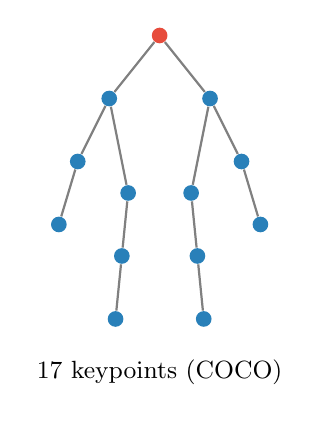
\begin{tikzpicture}[scale=0.8]
    % Skeleton
    \node[circle,fill=accent,inner sep=2pt] (nose) at (0,4) {};
    \node[circle,fill=probpose,inner sep=2pt] (ls) at (-0.8,3) {};
    \node[circle,fill=probpose,inner sep=2pt] (rs) at (0.8,3) {};
    \node[circle,fill=probpose,inner sep=2pt] (le) at (-1.3,2) {};
    \node[circle,fill=probpose,inner sep=2pt] (re) at (1.3,2) {};
    \node[circle,fill=probpose,inner sep=2pt] (lw) at (-1.6,1) {};
    \node[circle,fill=probpose,inner sep=2pt] (rw) at (1.6,1) {};
    \node[circle,fill=probpose,inner sep=2pt] (lh) at (-0.5,1.5) {};
    \node[circle,fill=probpose,inner sep=2pt] (rh) at (0.5,1.5) {};
    \node[circle,fill=probpose,inner sep=2pt] (lk) at (-0.6,0.5) {};
    \node[circle,fill=probpose,inner sep=2pt] (rk) at (0.6,0.5) {};
    \node[circle,fill=probpose,inner sep=2pt] (la) at (-0.7,-0.5) {};
    \node[circle,fill=probpose,inner sep=2pt] (ra) at (0.7,-0.5) {};
    % Connections
    \draw[thick,gray] (nose)--(ls) (nose)--(rs);
    \draw[thick,gray] (ls)--(le)--(lw) (rs)--(re)--(rw);
    \draw[thick,gray] (ls)--(lh) (rs)--(rh);
    \draw[thick,gray] (lh)--(lk)--(la) (rh)--(rk)--(ra);
    \node[below] at (0,-1) {\small 17 keypoints (COCO)};
\end{tikzpicture}
\end{column}
\end{columns}
\end{frame}

% ============================================================
% PART 2: HOW IT WORKS
% ============================================================
\section{Cara Kerja}

\begin{frame}{Pendekatan Top-Down}
\centering
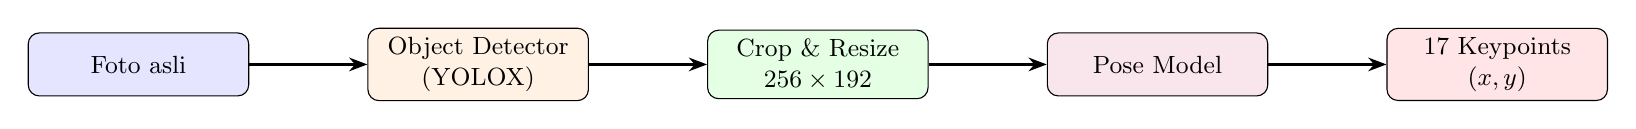
\begin{tikzpicture}[node distance=1.5cm, >=Stealth,
    box/.style={rectangle, draw, rounded corners, minimum width=2.8cm, minimum height=0.8cm, align=center, font=\small}]
    
    \node[box, fill=blue!10] (input) {Foto asli};
    \node[box, fill=orange!10, right=of input] (detect) {Object Detector\\(YOLOX)};
    \node[box, fill=green!10, right=of detect] (crop) {Crop \& Resize\\$256\times192$};
    \node[box, fill=purple!10, right=of crop] (model) {Pose Model};
    \node[box, fill=red!10, right=of model] (output) {17 Keypoints\\$(x, y)$};
    
    \draw[->,thick] (input) -- (detect);
    \draw[->,thick] (detect) -- (crop);
    \draw[->,thick] (crop) -- (model);
    \draw[->,thick] (model) -- (output);
\end{tikzpicture}

\vspace{1.5em}
\begin{itemize}
    \item Deteksi orang $\rightarrow$ Crop per orang $\rightarrow$ Estimasi pose per orang
    \item Akurasi tinggi karena fokus satu orang per inferensi
\end{itemize}
\end{frame}

\begin{frame}{Heatmap: Cara Model ``Menunjuk'' Lokasi Sendi}
\begin{columns}
\begin{column}{0.55\textwidth}
\begin{itemize}
    \item Model output \textbf{17 peta} (satu per sendi)
    \item Setiap peta berukuran $64\times48$
    \item Nilai tinggi = ``sendi kemungkinan di sini''
    \item Koordinat akhir = titik paling terang (\texttt{argmax})
\end{itemize}

\vspace{1em}
\textbf{Training:}\\
Target = Gaussian 2D di lokasi ground truth\\
Loss = MSE (Mean Squared Error)
\end{column}
\begin{column}{0.45\textwidth}
\centering
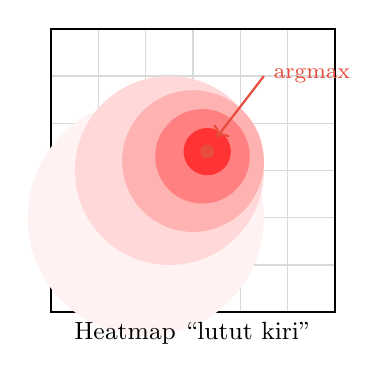
\begin{tikzpicture}[scale=0.6]
    \draw[step=1,gray!30,thin] (0,0) grid (6,6);
    \draw[thick] (0,0) rectangle (6,6);
    % Gaussian blob
    \fill[red!5] (2,2) circle (2.5);
    \fill[red!15] (2.5,3) circle (2);
    \fill[red!30] (3,3.2) circle (1.5);
    \fill[red!50] (3.2,3.3) circle (1);
    \fill[red!80] (3.3,3.4) circle (0.5);
    \fill[accent] (3.3,3.4) circle (0.15);
    \node[below,font=\small] at (3,0) {Heatmap ``lutut kiri''};
    \draw[->,thick,accent] (4.5,5) -- (3.5,3.7);
    \node[right,font=\footnotesize,accent] at (4.5,5) {argmax};
\end{tikzpicture}
\end{column}
\end{columns}
\end{frame}

% ============================================================
% PART 3: THE PROBLEMS
% ============================================================
\section{Masalah}

\begin{frame}{Masalah 1: Keypoint di Luar Gambar}
\begin{columns}
\begin{column}{0.45\textwidth}
\centering
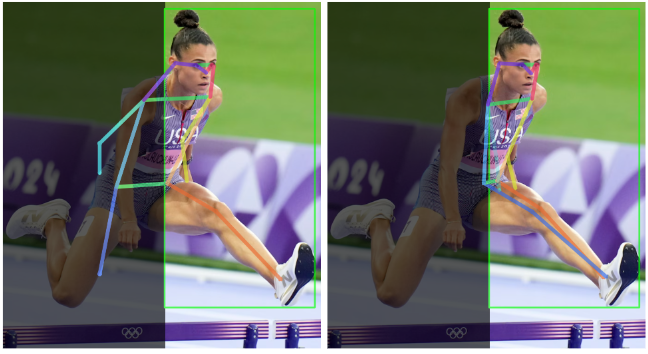
\includegraphics[width=\linewidth,height=0.7\textheight,keepaspectratio]{gambar/figure1.png}

{\tiny\textit{Figure 1: ProbPose (kiri) vs ViTPose (kanan)}}
\end{column}
\begin{column}{0.55\textwidth}
\textbf{Apa yang terjadi:}
\begin{itemize}
    \item Bounding box tidak selalu mencakup seluruh tubuh
    \item Beberapa sendi \textcolor{accent}{terpotong}
\end{itemize}

\vspace{1em}
\textbf{Model konvensional:}
\begin{itemize}
    \item Tidak bisa bilang ``tidak ada''
    \item Asal menebak lokasi $\rightarrow$ \textcolor{accent}{salah}
    \item Evaluasi (OKS) \textbf{mengabaikan} masalah ini
\end{itemize}

\vspace{0.5em}
{\small\textcolor{success}{ProbPose} memprediksi kaki kanan di luar gambar dengan benar. \textcolor{accent}{ViTPose} menempelkan kaki kanan ke kaki kiri.}
\end{column}
\end{columns}
\end{frame}

\begin{frame}{Masalah 2: Heatmap Tidak Terkalibrasi}
\begin{columns}
\begin{column}{0.5\textwidth}
\textbf{Heatmap konvensional:}
\begin{itemize}
    \item Nilai bukan probabilitas sesungguhnya
    \item Bentuk dipaksa Gaussian (sigma tetap)
    \item Tidak bisa mengekspresikan \textit{ketidakpastian}
\end{itemize}

\vspace{1em}
\textbf{Dampak:}
\begin{itemize}
    \item Tidak bisa jawab: ``seberapa yakin?''
    \item Berbahaya untuk aplikasi safety-critical
    \item Robot, self-driving, medis
\end{itemize}
\end{column}
\begin{column}{0.5\textwidth}
\centering
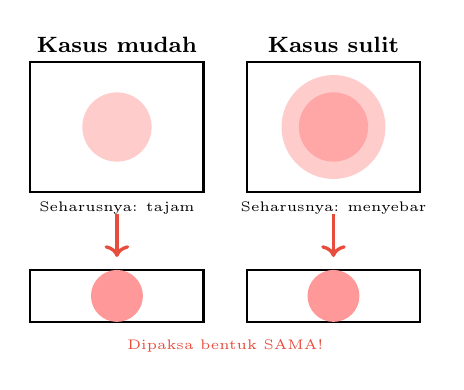
\begin{tikzpicture}[scale=0.55]
    % Case 1: certain
    \draw[thick] (0,3) rectangle (4,6);
    \node[above,font=\footnotesize\bfseries] at (2,6) {Kasus mudah};
    \fill[red!60] (2,4.5) circle (0.4);
    \fill[red!20] (2,4.5) circle (0.8);
    \node[below,font=\tiny] at (2,3) {Seharusnya: tajam};
    
    % Case 2: uncertain
    \draw[thick] (5,3) rectangle (9,6);
    \node[above,font=\footnotesize\bfseries] at (7,6) {Kasus sulit};
    \fill[red!20] (7,4.5) circle (1.2);
    \fill[red!35] (7,4.5) circle (0.8);
    \node[below,font=\tiny] at (7,3) {Seharusnya: menyebar};
    
    % Arrow
    \draw[->,very thick,accent] (2,2.5) -- (2,1.5);
    \draw[->,very thick,accent] (7,2.5) -- (7,1.5);
    
    % Forced same
    \draw[thick] (0,0) rectangle (4,1.2);
    \fill[red!40] (2,0.6) circle (0.6);
    \draw[thick] (5,0) rectangle (9,1.2);
    \fill[red!40] (7,0.6) circle (0.6);
    \node[below,font=\tiny,accent] at (4.5,-0.2) {Dipaksa bentuk SAMA!};
\end{tikzpicture}
\end{column}
\end{columns}
\end{frame}

% ============================================================
% PART 4: PROBPOSE SOLUTION
% ============================================================
\section{ProbPose}

\begin{frame}{ProbPose: Ide Utama}
\centering
\vspace{0.5em}
{\large Model konvensional hanya bisa bilang:}\\[0.3em]
{\Large\bfseries ``Sendi ada \textcolor{probpose}{DI SINI}.''}

\vspace{1.5em}
{\large ProbPose bisa bilang \textbf{4 hal}:}

\vspace{0.8em}
\begin{tabular}{cl}
\textcolor{probpose}{\textbf{1.}} & Di mana sendi ini? \textit{(Probability Map)} \\[0.5em]
\textcolor{probpose}{\textbf{2.}} & Apakah sendi ini ada di gambar? \textit{(Presence Score)} \\[0.5em]
\textcolor{probpose}{\textbf{3.}} & Seberapa bagus tebakan saya? \textit{(Quality Score)} \\[0.5em]
\textcolor{probpose}{\textbf{4.}} & Apakah sendi terlihat atau terhalang? \textit{(Visibility)} \\
\end{tabular}
\end{frame}

\begin{frame}{Arsitektur ProbPose}
\centering
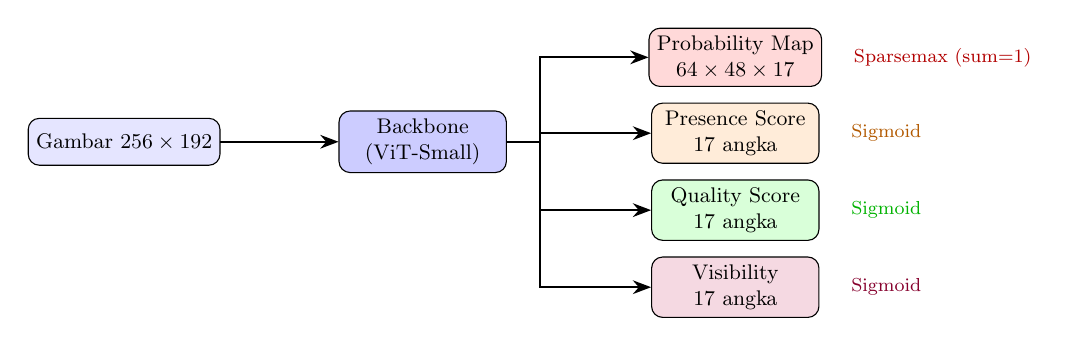
\begin{tikzpicture}[node distance=0.8cm, >=Stealth, scale=0.85, every node/.style={scale=0.85},
    box/.style={rectangle, draw, rounded corners, minimum width=2.5cm, minimum height=0.7cm, align=center, font=\small}]
    
    \node[box, fill=blue!10] (input) {Gambar $256\times192$};
    \node[box, fill=blue!20, right=1.5cm of input] (backbone) {Backbone\\(ViT-Small)};
    
    % Heads
    \node[box, fill=red!15, above right=0.3cm and 1.8cm of backbone] (h1) {Probability Map\\$64\times48\times17$};
    \node[box, fill=orange!15, below=0.2cm of h1] (h2) {Presence Score\\$17$ angka};
    \node[box, fill=green!15, below=0.2cm of h2] (h3) {Quality Score\\$17$ angka};
    \node[box, fill=purple!15, below=0.2cm of h3] (h4) {Visibility\\$17$ angka};
    
    \draw[->,thick] (input) -- (backbone);
    \draw[->,thick] (backbone.east) -- ++(0.5,0) |- (h1.west);
    \draw[->,thick] (backbone.east) -- ++(0.5,0) |- (h2.west);
    \draw[->,thick] (backbone.east) -- ++(0.5,0) |- (h3.west);
    \draw[->,thick] (backbone.east) -- ++(0.5,0) |- (h4.west);
    
    \node[right=0.3cm of h1,font=\footnotesize,red!70!black] {Sparsemax (sum=1)};
    \node[right=0.3cm of h2,font=\footnotesize,orange!70!black] {Sigmoid};
    \node[right=0.3cm of h3,font=\footnotesize,green!70!black] {Sigmoid};
    \node[right=0.3cm of h4,font=\footnotesize,purple!70!black] {Sigmoid};
\end{tikzpicture}
\end{frame}

\begin{frame}{Output 1: Probability Map}
\begin{columns}
\begin{column}{0.5\textwidth}
\textbf{Heatmap konvensional:}
\begin{itemize}
    \item Setiap piksel independen
    \item Total bisa berapa saja
    \item Bukan probabilitas
\end{itemize}

\vspace{1em}
\textbf{Probability Map (ProbPose):}
\begin{itemize}
    \item Semua piksel \textbf{berbagi 100\%}
    \item Total selalu = 1
    \item Probabilitas sesungguhnya
    \item Bentuk bebas (adaptif)
\end{itemize}
\end{column}
\begin{column}{0.5\textwidth}
\centering
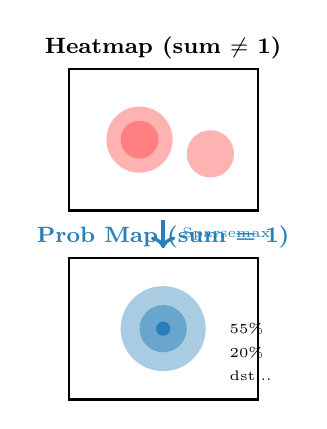
\begin{tikzpicture}[scale=0.6]
    % Heatmap
    \draw[thick] (0,4) rectangle (4,7);
    \node[above,font=\footnotesize\bfseries] at (2,7) {Heatmap (sum $\neq$ 1)};
    \fill[red!30] (1.5,5.5) circle (0.7);
    \fill[red!50] (1.5,5.5) circle (0.4);
    \fill[red!30] (3,5.2) circle (0.5);
    
    % Prob map
    \draw[thick] (0,0) rectangle (4,3);
    \node[above,font=\footnotesize\bfseries,probpose] at (2,3) {Prob Map (sum = 1)};
    \fill[probpose!40] (2,1.5) circle (0.9);
    \fill[probpose!70] (2,1.5) circle (0.5);
    \fill[probpose] (2,1.5) circle (0.15);
    \node[right,font=\tiny] at (3.2,1.5) {55\%};
    \node[right,font=\tiny] at (3.2,1) {20\%};
    \node[right,font=\tiny] at (3.2,0.5) {dst...};
    
    \draw[->,very thick,probpose] (2,3.8) -- (2,3.2);
    \node[right,font=\tiny,probpose] at (2.2,3.5) {Sparsemax};
\end{tikzpicture}
\end{column}
\end{columns}
\end{frame}

\begin{frame}{Output 2: Presence Score}
\centering
\vspace{0.5em}
{\large ``Apakah sendi ini \textbf{ada} di dalam gambar?''}

\vspace{1.5em}
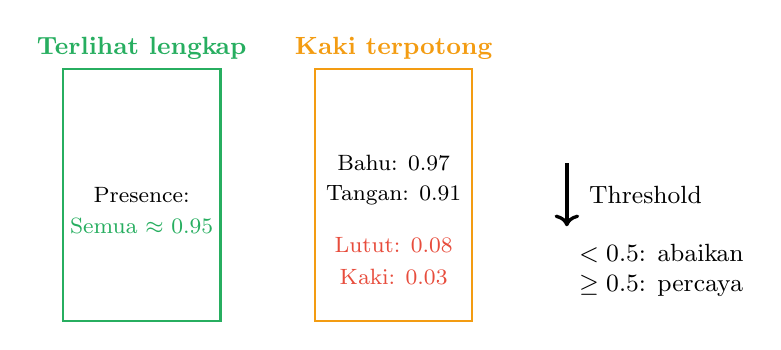
\begin{tikzpicture}[scale=0.8]
    % Image with full body
    \draw[thick,success] (0,0) rectangle (2.5,4);
    \node[above,font=\small\bfseries,success] at (1.25,4) {Terlihat lengkap};
    \node[font=\footnotesize] at (1.25,2) {Presence:};
    \node[font=\footnotesize,success] at (1.25,1.5) {Semua $\approx$ 0.95};
    
    % Image with cropped legs
    \draw[thick,warning] (4,0) rectangle (6.5,4);
    \node[above,font=\small\bfseries,warning] at (5.25,4) {Kaki terpotong};
    \node[font=\footnotesize] at (5.25,2.5) {Bahu: 0.97};
    \node[font=\footnotesize] at (5.25,2) {Tangan: 0.91};
    \node[font=\footnotesize,accent] at (5.25,1.2) {Lutut: 0.08};
    \node[font=\footnotesize,accent] at (5.25,0.7) {Kaki: 0.03};
    
    % Arrow
    \draw[->,very thick] (8,2.5) -- (8,1.5);
    \node[right,font=\small] at (8.2,2) {Threshold};
    \node[font=\small,align=left] at (9.5,0.8) {$< 0.5$: abaikan\\$\geq 0.5$: percaya};
\end{tikzpicture}

\vspace{1em}
\textbf{Model konvensional tidak punya kemampuan ini.}
\end{frame}

\begin{frame}{Output 3 \& 4: Quality Score \& Visibility}
\begin{columns}
\begin{column}{0.5\textwidth}
\textbf{Quality Score:}\\[0.5em]
``Seberapa bagus tebakan lokasi saya?''

\vspace{0.5em}
\begin{itemize}
    \item Self-assessment model
    \item Ditraining terhadap OKS sesungguhnya
    \item Terkalibrasi (angka bermakna)
    \item Berguna saat inferensi (tanpa ground truth)
\end{itemize}
\end{column}
\begin{column}{0.5\textwidth}
\textbf{Visibility:}\\[0.5em]
``Apakah sendi terlihat atau terhalang?''

\vspace{0.5em}
\begin{itemize}
    \item Visible: terlihat langsung
    \item Occluded: ada tapi ketutupan
    \item Target dari anotasi COCO
    \item Berbeda dari presence (posisi vs halangan)
\end{itemize}
\end{column}
\end{columns}

\vspace{1em}
\centering
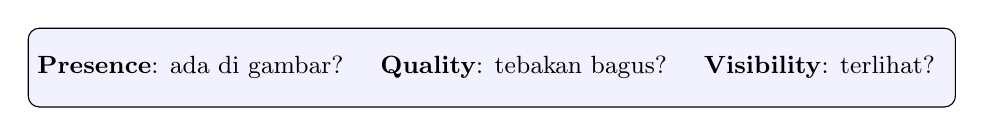
\begin{tikzpicture}
\node[draw,rounded corners,fill=blue!5,minimum width=10cm,minimum height=1cm,align=center,font=\small] {
    \textbf{Presence}: ada di gambar? \quad
    \textbf{Quality}: tebakan bagus? \quad
    \textbf{Visibility}: terlihat?
};
\end{tikzpicture}
\end{frame}

\begin{frame}{Loss Functions}
\centering
\vspace{0.5em}
\textbf{4 output $\rightarrow$ 4 loss function}

\vspace{1em}
\begin{tabular}{lll}
\toprule
\textbf{Output} & \textbf{Loss} & \textbf{Target} \\
\midrule
Probability Map & OKS Heatmap Loss & OKS map \\
Presence Score & Binary Cross Entropy & 0 atau 1 \\
Quality Score & MSE & Skor OKS sesungguhnya \\
Visibility & Binary Cross Entropy & 0 atau 1 \\
\bottomrule
\end{tabular}

\vspace{1.5em}
$$\mathcal{L}_{total} = \mathcal{L}_{OKS} + \mathcal{L}_{presence} + \mathcal{L}_{quality} + \mathcal{L}_{visibility}$$

\vspace{0.5em}
{\small Semua head ditraining bersamaan, tapi hanya heatmap head yang melatih backbone.}
\end{frame}

\begin{frame}{OKS: Object Keypoint Similarity}
\begin{columns}
\begin{column}{0.55\textwidth}
\textbf{Metrik evaluasi utama} untuk pose estimation:

$$\text{OKS} = \exp\left(\frac{-d^2}{2 \cdot s^2 \cdot k^2}\right)$$

\begin{itemize}
    \item $d$ = jarak prediksi vs ground truth
    \item $s$ = skala (ukuran orang)
    \item $k$ = konstanta per keypoint
\end{itemize}

\vspace{0.5em}
Nilai: $0$ (salah total) $\rightarrow$ $1$ (sempurna)
\end{column}
\begin{column}{0.45\textwidth}
\centering
\textbf{Toleransi berbeda per sendi:}

\vspace{0.5em}
\begin{tabular}{ll}
\footnotesize Hidung & \footnotesize $k$ kecil (ketat) \\
\footnotesize Bahu & \footnotesize $k$ sedang \\
\footnotesize Pinggul & \footnotesize $k$ besar (longgar) \\
\end{tabular}

\vspace{1em}
{\small Karena variasi antar-anotator manusia berbeda per sendi.}
\end{column}
\end{columns}
\end{frame}

\begin{frame}{Expected OKS Maximization (Decoding)}
\begin{columns}
\begin{column}{0.45\textwidth}
\textbf{Konvensional (argmax/UDP):}
\begin{itemize}
    \item Ambil titik tertinggi
    \item Refine lokal
    \item Bisa tertipu oleh spike tajam
\end{itemize}

\vspace{1em}
\textbf{ProbPose (Expected OKS):}
\begin{itemize}
    \item Hitung expected OKS per piksel
    \item Pilih yang memaksimalkan skor
    \item Lebih robust untuk distribusi bimodal
\end{itemize}
\end{column}
\begin{column}{0.55\textwidth}
\centering
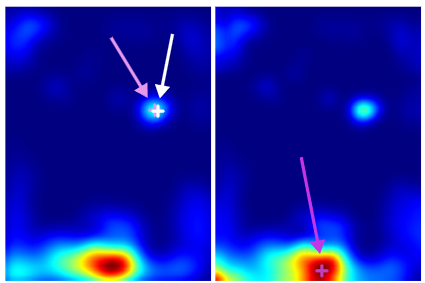
\includegraphics[width=\linewidth,height=0.7\textheight,keepaspectratio]{gambar/figure3.png}

{\tiny\textit{Figure 3: UDP decoding (kiri) vs Expected OKS maximization (kanan)}}
\end{column}
\end{columns}
\end{frame}

% ============================================================
% PART 5: EVALUATION
% ============================================================
\section{Evaluasi Baru}

\begin{frame}{CropCOCO Dataset}
\begin{columns}
\begin{column}{0.5\textwidth}
\textbf{Masalah:}\\
COCO biasa jarang punya keypoint di luar gambar $\rightarrow$ tidak bisa mengukur kemampuan model.

\vspace{1em}
\textbf{Solusi: CropCOCO}\\
Gambar COCO di-crop lebih agresif sehingga banyak keypoint jatuh di luar frame.

\vspace{1em}
\textbf{Tujuan:}\\
Mengukur kemampuan model menangani out-of-image keypoints.
\end{column}
\begin{column}{0.5\textwidth}
\centering
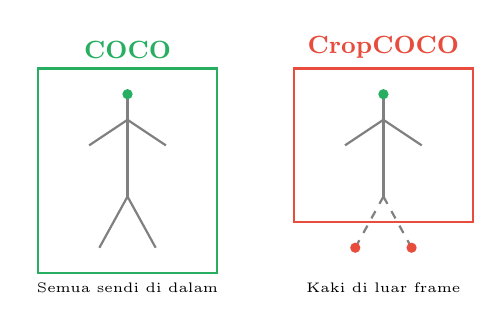
\begin{tikzpicture}[scale=0.65]
    % COCO normal
    \draw[thick,success] (0,3) rectangle (3.5,7);
    \node[above,font=\small\bfseries,success] at (1.75,7) {COCO};
    % stick figure inside
    \draw[gray,thick] (1.75,6.5) -- (1.75,4.5);
    \draw[gray,thick] (1.75,6) -- (1,5.5) (1.75,6) -- (2.5,5.5);
    \draw[gray,thick] (1.75,4.5) -- (1.2,3.5) (1.75,4.5) -- (2.3,3.5);
    \fill[success] (1.75,6.5) circle (0.1);
    \node[below,font=\tiny] at (1.75,3) {Semua sendi di dalam};
    
    % CropCOCO
    \draw[thick,accent] (5,4) rectangle (8.5,7);
    \node[above,font=\small\bfseries,accent] at (6.75,7) {CropCOCO};
    % stick figure partially outside
    \draw[gray,thick] (6.75,6.5) -- (6.75,4.5);
    \draw[gray,thick] (6.75,6) -- (6,5.5) (6.75,6) -- (7.5,5.5);
    \draw[gray,thick,dashed] (6.75,4.5) -- (6.2,3.5) (6.75,4.5) -- (7.3,3.5);
    \fill[success] (6.75,6.5) circle (0.1);
    \fill[accent] (6.2,3.5) circle (0.1);
    \fill[accent] (7.3,3.5) circle (0.1);
    \node[below,font=\tiny] at (6.75,3) {Kaki di luar frame};
\end{tikzpicture}
\end{column}
\end{columns}
\end{frame}

\begin{frame}{Ex-OKS: Extended OKS}
\centering
\vspace{0.5em}
{\large OKS biasa \textbf{mengabaikan} keypoint di luar gambar.\\Ex-OKS \textbf{menghukum} false positive.}

\vspace{1em}
\begin{tabular}{lcc}
\toprule
\textbf{Situasi} & \textbf{OKS} & \textbf{Ex-OKS} \\
\midrule
KP di dalam + prediksi benar & skor tinggi & skor tinggi \\
KP di dalam + prediksi salah & skor rendah & skor rendah \\
KP di luar + model bilang ``tidak ada'' & \textcolor{gray}{diabaikan} & \textcolor{success}{skor tinggi} \\
KP di luar + model bilang ``ada'' & \textcolor{gray}{diabaikan} & \textcolor{accent}{skor rendah} \\
\bottomrule
\end{tabular}

\vspace{1.5em}
\textbf{Ex-OKS menghargai model yang jujur bilang ``tidak tahu.''}
\end{frame}

% ============================================================
% PART 6: RESULTS
% ============================================================
\section{Hasil Eksperimen}

\begin{frame}{Hasil: Perbandingan dengan SOTA}
\centering
\vspace{0.3em}
{\small Semua model berukuran serupa. Evaluasi menggunakan GT bounding boxes.}

\vspace{0.8em}
\begin{tabular}{l|cc|cc|cc}
\toprule
& \multicolumn{2}{c|}{\textbf{COCO}} & \multicolumn{2}{c|}{\textbf{CropCOCO}} & \multicolumn{2}{c}{\textbf{OCHuman}} \\
\textbf{Model} & mAP & Ex-mAP & mAP & Ex-mAP & mAP & Ex-mAP \\
\midrule
ViTPose-s & 75.9 & 75.3 & 72.7 & 66.5 & 60.3 & 60.1 \\
HRFormer-s & 75.2 & 74.6 & 70.9 & 64.3 & 60.3 & 60.0 \\
SWIN-t & 73.5 & 72.9 & 71.3 & 65.0 & 58.1 & 57.9 \\
\midrule
\textbf{ProbPose-s} & \textbf{76.6} & \textbf{76.4} & \textbf{81.7} & \textbf{73.9} & 60.4 & 60.2 \\
\bottomrule
\end{tabular}

\vspace{1em}
\begin{itemize}
    \item COCO: peningkatan kecil (+0.7\% vs ViTPose)
    \item \textcolor{success}{\textbf{CropCOCO: peningkatan signifikan (+9.0\%)}} $\leftarrow$ kontribusi utama
    \item OCHuman: kompetitif
\end{itemize}
\end{frame}

\begin{frame}{Ablation Study}
\centering
\vspace{0.5em}
{\small Apa yang paling berkontribusi?}

\vspace{1em}
\begin{tabular}{cc|cc}
\toprule
\textbf{Prob. Map} & \textbf{Crop Aug.} & \textbf{COCO mAP} & \textbf{CropCOCO mAP} \\
\midrule
\texttimes & \texttimes & 76.0 & 73.7 \\
\texttimes & \checkmark & 76.4 & 72.4 \\
\checkmark & \texttimes & 76.6 & 81.7 \\
\checkmark & \checkmark & \textbf{76.6} & \textbf{81.7} \\
\bottomrule
\end{tabular}

\vspace{1.5em}
\textbf{Temuan:}
\begin{itemize}
    \item Crop augmentation = kontributor utama untuk CropCOCO
    \item Probability map = keunggulan di versatility, bukan akurasi murni
    \item Kombinasi keduanya = hasil terbaik
\end{itemize}
\end{frame}

\begin{frame}{Presence Probability vs Confidence}
\begin{columns}
\begin{column}{0.5\textwidth}
\textbf{Klasifikasi in/out-of-image:}

\vspace{0.5em}
\begin{itemize}
    \item ProbPose presence probability\\mengurangi error \textbf{30--45\%}\\dibanding confidence ViTPose
    \item Confidence tidak ditraining untuk tugas ini
    \item Threshold optimal: 0.15--0.4\\(bukan 0.3 yang umum dipakai)
\end{itemize}
\end{column}
\begin{column}{0.5\textwidth}
\centering
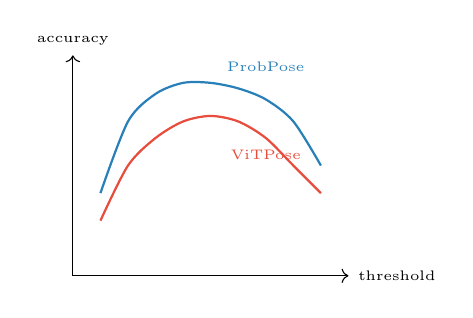
\begin{tikzpicture}[scale=0.7]
    \draw[->] (0,0) -- (5,0) node[right,font=\tiny] {threshold};
    \draw[->] (0,0) -- (0,4) node[above,font=\tiny] {accuracy};
    % ProbPose curve (higher)
    \draw[thick,probpose] plot[smooth] coordinates {(0.5,1.5) (1,2.8) (1.5,3.3) (2,3.5) (2.5,3.5) (3,3.4) (3.5,3.2) (4,2.8) (4.5,2)};
    % ViTPose curve (lower)
    \draw[thick,accent] plot[smooth] coordinates {(0.5,1) (1,2) (1.5,2.5) (2,2.8) (2.5,2.9) (3,2.8) (3.5,2.5) (4,2) (4.5,1.5)};
    \node[font=\tiny,probpose] at (3.5,3.8) {ProbPose};
    \node[font=\tiny,accent] at (3.5,2.2) {ViTPose};
\end{tikzpicture}
\end{column}
\end{columns}
\end{frame}

% ============================================================
% PART 7: LIMITATIONS & CONCLUSION
% ============================================================
\section{Limitasi \& Kesimpulan}

\begin{frame}{Limitasi}
\begin{enumerate}
    \item \textbf{Peningkatan in-image kecil} (+0.7\% di COCO)\\
    {\small Untuk kasus normal, manfaat minimal}
    
    \vspace{0.5em}
    \item \textbf{Hanya model Small}\\
    {\small Belum diuji pada backbone besar (ViTPose-L, -H)}
    
    \vspace{0.5em}
    \item \textbf{Multi-person belum dieksplorasi}\\
    {\small Crowded scene dengan banyak orang tumpang tindih}
    
    \vspace{0.5em}
    \item \textbf{Bergantung pada crop augmentation}\\
    {\small Tanpa itu, probability map justru menurunkan performa}
    
    \vspace{0.5em}
    \item \textbf{Anotasi COCO bermasalah di tepi}\\
    {\small Model dihukum karena lebih akurat dari ground truth}
\end{enumerate}
\end{frame}

\begin{frame}{Kesimpulan}
\begin{columns}
\begin{column}{0.6\textwidth}
\textbf{Kontribusi ProbPose:}
\begin{enumerate}
    \item \textbf{Probability map} $\rightarrow$ distribusi terkalibrasi (sum=1)
    \item \textbf{Presence probability} $\rightarrow$ error turun 45\%
    \item \textbf{OKS-based loss} $\rightarrow$ training selaras dengan evaluasi
    \item \textbf{CropCOCO + Ex-OKS} $\rightarrow$ evaluasi yang lebih lengkap
    \item \textbf{Crop augmentation} $\rightarrow$ +9\% di out-of-image
\end{enumerate}

\vspace{1em}
\textbf{Pesan utama:}\\
{\small Pose estimation bukan hanya soal akurasi lokalisasi, tapi juga soal \textit{kejujuran} model --- tahu kapan harus bilang ``tidak tahu.''}
\end{column}
\begin{column}{0.4\textwidth}
\centering
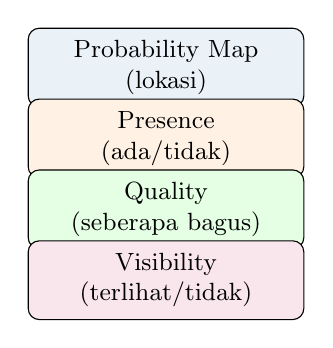
\begin{tikzpicture}[scale=0.6]
    \node[draw,rounded corners,fill=probpose!10,minimum width=3.5cm,minimum height=1cm,align=center,font=\small] at (0,3) {Probability Map\\(lokasi)};
    \node[draw,rounded corners,fill=orange!10,minimum width=3.5cm,minimum height=1cm,align=center,font=\small] at (0,1.5) {Presence\\(ada/tidak)};
    \node[draw,rounded corners,fill=green!10,minimum width=3.5cm,minimum height=1cm,align=center,font=\small] at (0,0) {Quality\\(seberapa bagus)};
    \node[draw,rounded corners,fill=purple!10,minimum width=3.5cm,minimum height=1cm,align=center,font=\small] at (0,-1.5) {Visibility\\(terlihat/tidak)};
\end{tikzpicture}
\end{column}
\end{columns}
\end{frame}

% ============================================================
% DEMO & REFERENCES
% ============================================================
\section{Demo}

\begin{frame}{Demo: Implementasi}
\centering
\vspace{0.5em}
\textbf{Stack yang digunakan:}

\vspace{1em}
\begin{tabular}{ll}
\toprule
Framework & MMPose (OpenMMLab) \\
Backbone & Vision Transformer Small (ViT-S) \\
Head & ProbMapHead (custom) \\
Input & $256 \times 192$ \\
Output & $64 \times 48 \times 17$ probability maps \\
Weights & ProbPose-s.pth (pre-trained) \\
Detector & YOLOX (untuk multi-person) \\
\bottomrule
\end{tabular}

\vspace{1.5em}
{\small Kode tersedia di: \texttt{github.com/MiraPurkrabek/ProbPose\_code}}
\end{frame}

\begin{frame}{}
\centering
\vspace{2cm}
{\Huge\bfseries Terima Kasih}

\vspace{1.5em}
{\large Pertanyaan?}

\vspace{2em}
{\small
Paper: \textit{ProbPose: A Probabilistic Approach to 2D Human Pose Estimation}\\
Purkrabek \& Matas, CVPR 2025\\[0.5em]
\texttt{arxiv.org/abs/2412.02254}
}
\end{frame}

\end{document}
